\documentclass[10pt,twocolumn]{article}
\usepackage{amsthm, amssymb, geometry, mathrsfs}
\usepackage[T1]{fontenc}
\usepackage{graphicx}
\usepackage[utf8]{inputenc}
\usepackage[style=ieee]{biblatex}
\addbibresource{citations.bib}
\usepackage{multicol}% http://ctan.org/pkg/multicols

\title {COMP 598: Multi-Class Classification of Reddit comments.}
\author {Xavier Denis, Ian Forbes, Liu Liu}

\begin {document}

\twocolumn[
\maketitle
\section{Abstract}
We collect a new machine learning dataset from the online social network Reddit. Consisting of the Top 100 posts from 2014, along with their comments from  the 10 most popular subreddits. We implement a Naive Bayes classifier to classify the subreddit which the comment belongs. The binary classification performance of  Naive Bayes reaches 89\% after 10-fold cross validation with around 80,000 comments. The multi-class classification performance with 6 classes using 35k-94k comments per class is 50\%. This work shows the possibility of recommending comment automatically based off of a user's comment history on Reddit.
\\
\\
]
\section{What is Reddit?}

Reddit is a popular online link aggregation website. It allows user to both post links to other webpages, images, videos, and more and to vote on the popularity of these submissions. Popular submissions are `Upvoted' while unpopular ones are `Downvoted'. Users are also allowed to comment on and discuss submissions. Comments, like submissions, are also voted on. Some of the key vocabulary of Reddit is listed below.

\begin {enumerate}
\item \textbf{Post:} Also know as a submission is a link to another webpage. This webpage may be a news article, a blog post, an image, a video, etc. All posts contain a comment section where user are allowed to discuss the submission.
\item \textbf{Self Post:} Is a special type of post where a user writes their own text submission. This is often used to started discussions or ask questions in a given subreddit. 
\item \textbf{Subreddit:} A subsection of Reddit dedicated to a certain topic. 
\item \textbf{Upvote \& Downvote:} The action of voting on the popularity of a comment in either a positive or negative manner.
\item \textbf{Top level comment:} The root of a comment tree.
\end {enumerate}

\section{Motivation}
With the rise of social networks, many researchers have poured over the data produced to find explore the connections between friends, text, and social interactions. While much research has been done on networks such as Twitter and Facebook, Reddit has remained largely ignored. The different structure of Reddit allows for an opportunity to look at different questions and a different style of conversation. Because Reddit users can label comments and posts as good or bad through voting, we can attempt to predict the interests of Reddit users.

Reddit also offers easy access to data for research and non-commercial purposes through it's API.\cite{Reddit}. 

\begin{figure*}
    \centering
  	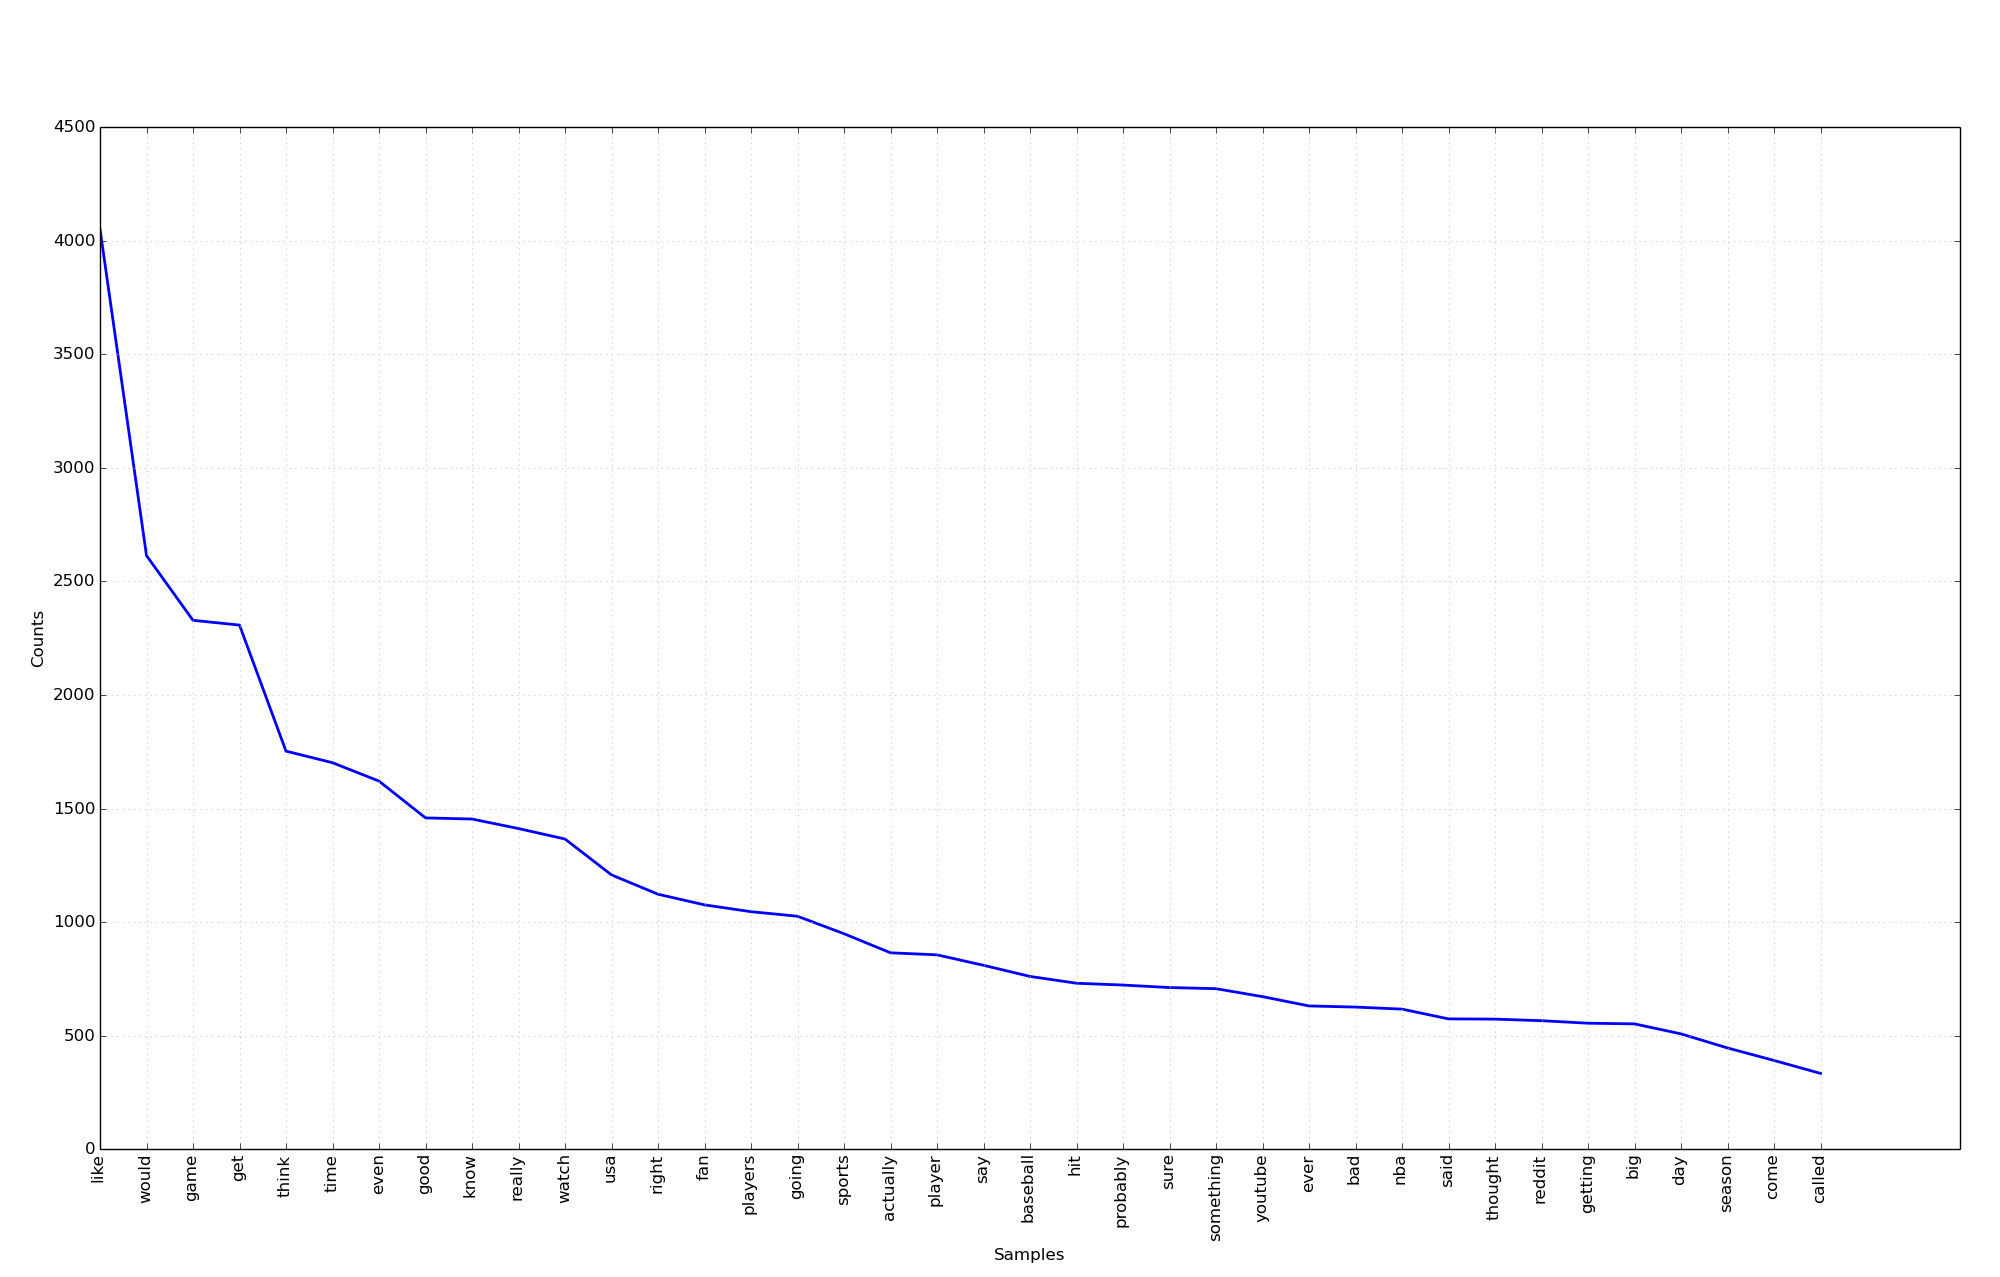
\includegraphics[width=0.92\textwidth]{./sports_freq.png}
  	\caption{Word frequency of the Sports subreddit.}
  	\label{sports}
\end{figure*}

\section{Related Work}

Due to the lack of studies related to Reddit there are few related datasets or papers. A search through Google Scholar produces few results and the top links are only listed because of share buttons on the paper's hosting site. Most of the related research we found were University projects like our own. We could not find any published papers or data.

However, we did find an interesting analysis that aimed to predict the popularity of a self post based on its Flesch-Kincaid\cite{flesch1949art} readability. This project found a correlation between how easy a self post was to read and how popular it would be. In particular posts with moderate readability where more popular than others with easy or hard readability.

Our classification problem also has a stark resemblance to the 20 news groups problem of \cite{joachims1996probabilistic}. This paper is the original 20 news groups paper and compares the performance of various classification algorithms. The paper presents a Text Frequency - Inverse Document Frequency (TF-IDF) algorithm as well a probabilistic variation on this algorithm. The authors compared the performance of these two algorithms, along with a naive Bayes classifier, to gauge their relative performance. In the end the performance of the algorithms was as follows.
\\

\begin{tabular}{|c|c|}
\hline
Probabilistic TF-IDF & 90.3 \\
Naive Bayes & 88.6 \\
TD-IDF & 82.3 \\
\hline
\end{tabular}

\section{Dataset Description}

Reddit's developer API allowed us to download all of the post and comment data into structured JSON files. Each post is saved in a JSON file under its primary identifier. Each data file consists of 2 main parts, the meta data and the comments. The meta data contains information about the post, such as how many comments there are, the score of the post, a link to the content and the type of content (image, video, article, etc.). The comments section consists of a list the top level comments for that post. Each of the top level comments contains a list of of child comments (replies) which in turn may have their own children. 

In order to train our naive Bayes classifier we had to flatten the comments and evaluate the global word frequency for all the posts, creating a unigram frequency matrix for each post with comments as rows and features as columns.

\section{Methods}

We used a Naive Bayes classifier with single words (unigrams) as the features. We choose this classifier with the given feature set because the feature space, all words, is extremely large. Given that naive Bayes' complexity is linear with respect to the number of features we believe this to be a good choise. Our choice of feature set stems from the simplicity and speed of extracting single words from the text. This consisted of splitting the text on spaces and removing punctuation. 

Other possible features sets that we considered but were not adopted were bigrams and term frequency–inverse document frequency (TF-IDF)\cite{salton1983introduction}. One of the difficulties with bigrams is that they increase the sparseness of the features. This fact couple with the nature of most reddit comments, short - with poor spelling, grammar, and punctuation, weighed against the perceived usefulness of bi-grams when compared to uni-grams.

The other feature set we considered  was TF-IDF. This compares the ratio between the frequency of a word in a document and its total frequency in the text corpus. This gives use another way to calculate the word frequency but penalizes words which are common among all documents in the corpus. Unfortunately we only learned of this method towards the deadline and did not have time to implement it.

The naive Bayes classifier is a simple probabilistic classifier that relies on Bayes' rule and the assumption that features are conditional independent. While this assumption is grossly inaccurate, it has been shown to be quite accurate. The output of the classifier the probability that a given set of features $f_1,f_2,...f_n$ belong to the class $C$. 

\[ Pr(C|f_1,f_2,...f_n) = \frac{Pr(C) \cdot Pr(f_1,f_2,...f_n|C)}{Pr(f_1,f_2,...,f_n)} \]

Therefore, the combination of words will not likely to appear in the text data to generate models of P(x|y) and apply generative learning (e.g. LDA) to text data classification.
Naive Bayes assume the $x$ are conditionally independent given $y$ and simplifies the problem.\autocite{jordan2002discriminative}

\subsection*{Multi-class classification}
We used a single classifier to compute P(y|x) for each class, and selected the class with highest probability.
The other option is to use k different 1-vs-all binary classifiers. However, this method is computationally slower since many classifiers need to be learned, and the binary classes are imbalanced as the target class has relatively fewer data points compared to the aggregation of all the other classes.

Laplace smoothing was applied since some words are not observed in the training data. The maximum likelihood estimator was,
\[
P(x_j|y=1) = \frac {\#[x_j=1 \land y=1]+1}{\#[y=1]+2}
\]
Therefore, if there are no words from that class, the prior probability will be $0.5$, this prior avoids making any assumptions about the likelyhood of observing a word in the dataset.

\begin{figure}
    \centering  
    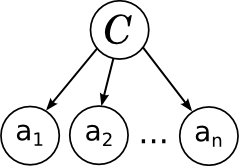
\includegraphics[width=0.5\textwidth]{./sysmag_bayes.png}
    \caption{Graphical representation of dependance in the Naive Bayes model. $C$ is the class and $a_i$ are the features. Readers should note that $C$ is dependent of the features but there is no dependence between features. }
    \label{bayesnet}
\end{figure}

Once all the features for the class were collected, we used a single classifier to compute P(y|x) for each class, selecting the highest probability class. The other option is to use $k$ different 1-vs-all binary classifiers. However, this method is computationally slower since many classifiers need to be learned, and the binary classes are imbalanced as the target class has relatively fewer data points compared to the aggregation of all the other classes.

To validate our results we performed 10-fold cross validation on our classifier (Fig \ref{multiclass}).
\section{Results}
\begin{figure}
    \centering
  	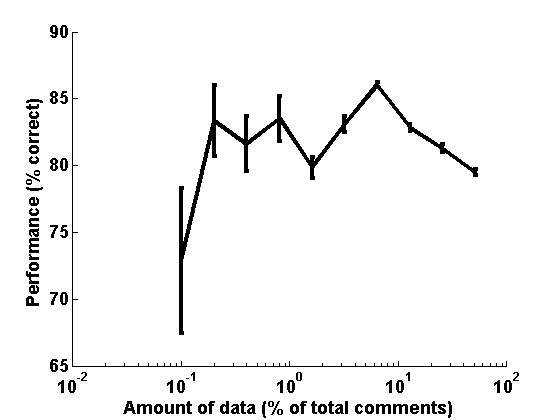
\includegraphics[width=0.5\textwidth]{./binary_data.png}
  \caption{ Binary classification performance as a function of the amount of data. There were a total of 35000 and 45000 comments in the two subreddits sports and books respectively. The performance was measure by 10-fold cross validation on the test data. The error bars represent the standard error of the 10 samples collected in the cross validation.}
  	\label{multiclass}
    \end{figure}
We measured good classification performance, attaining approximately $80\%$ performance (Fig \ref{multiclass}) when looking at the binary classification of two groups. As the amount of classes increased, the performance dropped but stayed well above that of a random classifier (Fig \ref{classes}). Most importantly, by using a single classifier we avoided biasing the results towards any one class, resulting in a fairly uniform confusion matrix (Fig \ref{confusion}). The amount of data in each class varied a lot but from this matrix we can see that there is no one class that was significantly more fitted than the others. 


\begin{figure}
    \centering
  	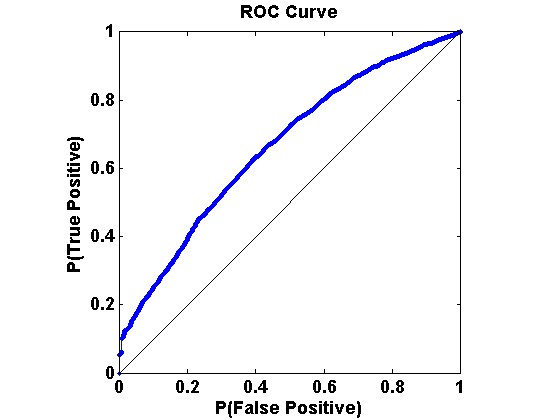
\includegraphics[width=0.5\textwidth]{./roc.png}
  	\caption{Receiver-operator characteristics (ROC) curve for binary classification performance using all the data. The classification threshold, i.e. decision boundary, of the naive Bayes classifier was defined by the log posterior of the test data.}
  	\label{roc}
\end{figure}		

\begin{figure}
    \centering
  	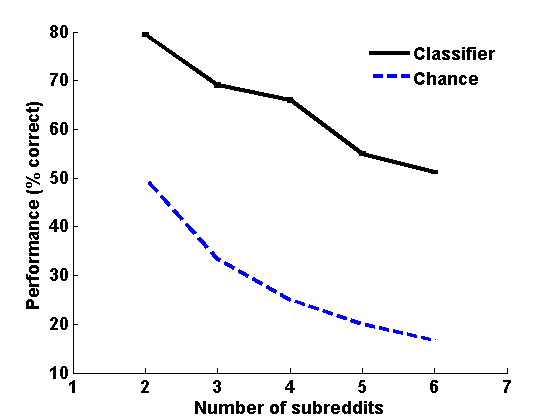
\includegraphics[width=0.5\textwidth]{./varyWBaseline.png}
  	\caption{Classifier performance as class count increases.}
  	\label{classes}
\end{figure}	

\begin{figure}
    \centering
  	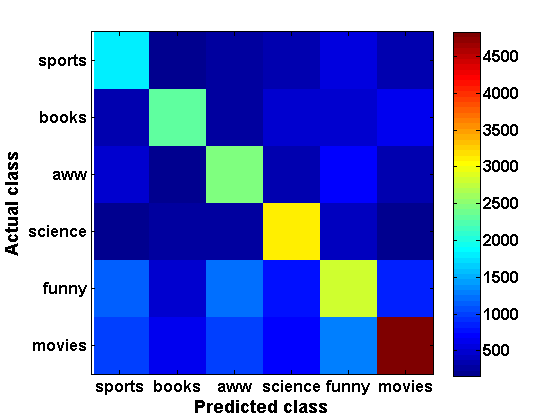
\includegraphics[width=0.5\textwidth]{./confusion_mat.png}
  	\caption{Confusion matrix for the multi-class performance. The number of comments in each subreddits is 35000, 45000, 46000, 46000, 73000, and 94000, respectively.}
  	\label{confusion}
\end{figure}	

\section{Discussion}
The final dataset and features are accurate when classifying but could still be improved. There were several issues during tokenization where standard approaches would fail due to Reddit's internal culture. The frequent use of non-textual unicode characters to encode emojis and other information wouldn't be captured by pure word tokenization. Additionally, the presence of Markdown for text formatting adds another level of complexity to the word extraction. We settled on stripping markdown formatting through regexes before splitting on spaces and stemming words. However, there a few issues with things such as `l33tspeak' where numbers are subsistuted for letters, causing use to not recognize identical words. 

Overall our results were quite positive. On possible use of our classifier would be to recommend new subreddits to users based on their comment history. Each user's comments are publicly available on their profile so it would be very easy to classify each of the comments into a given subreddit. If a user's comments where consistently classified into a small subset of subreddits it is possble that they may be interested in that subreddit. On a larger scale, sometimes posts are added to the wrong subreddit, this classifier could detect that comments really belong in a different subreddit and automatically move the entire post to that subreddit where it could receive the appropriate community interaction.

We hereby state that all the work presented in the report is that of the authors.

\section{References}
\printbibliography
\section{Appendix}

\end{document}